\section{Auswertung}
\label{sec:Auswertung}

Die folgende Auswertung wurde mit den Python Paketen numpy \cite{numpy}, scipy \cite{scipy} und matplotlib \cite{matplotlib} durchgeführt. 
\newline
Die Wellenlänge des Lichts des verwendeten Lasers beträgt
\begin{equation*}
    \lambda = \SI{532}{\nano\meter}.
\end{equation*}
% Tabelle mit Länge, Spannung 1, Zeit 1, Spannung 2 und Zeit 2 
%Grafik mit diesen Werten, also Screenshots 
\subsection{Beugung am ersten Einzelspalt}
In Tab. \ref{taba} werden die $x$-Koordinaten in Einheiten der Messanzeige und die Amplituden der Stromstärke gegeneinander aufgetragen. 

\begin{table}\caption{Die Länge der Zylinder und die Spannung mit den jeweiligen Zeitenpunkten der Ausschläge.}
\label{taba}
\centering
\sisetup{round-mode = places, round-precision=2, round-integer-to-decimal=true}
\begin{tabular}{S[]S[]S[]S[]S[]} 
\toprule
{$l/ \si{\milli\meter}$} & {$U_1/ \si{\volt}$} & {$t_1/ \si{\micro\second}$} & {$U_2/ \si{\volt}$} & {$t_2/ \si{\micro\second}$}\\
\midrule
120.8 & 1.29 & 0.6 & 0.17 & 88.7\\
102.3 & 1.27 & 0.5 & 0.2 & 76.5\\
80.5 & 1.33 & 0.6 & 0.76 & 59.8\\
40.4 & 1.33 & 0.5 & 1.34 & 30.2\\
31.1 & 1.29 & 0.5 & 1.37 & 23.8\\
\bottomrule
\end{tabular}\end{table}

\noindent In Tab. \ref{tab1} werden die $x$-Koordinaten mit Gleichung \eqref{eqn:phi} in Winkel umgerechnet und gegen die Amplitude der Stromstärke aufgetragen.

\begin{table}\caption{Der maximale Drehimpuls $L$, der Gesamtspin $S$ und der Gesamtdrehimpuls $J$ ergeben sich zum Landé-Faktor $g_\text{J}$ für die vier verschiedenen Elemente.}
\label{tab1}
\centering
\sisetup{round-mode = places, round-precision=2, round-integer-to-decimal=true}
\begin{tabular}{S[]S[]S[]S[]} 
\toprule
{$L$} & {$S$} & {$J$} & {$g_\text{J}$}\\
\midrule
5.0 & 1.0 & 4.0 & 0.8\\
0.0 & 3.5 & 3.5 & 2.0\\
6.0 & 1.5 & 4.5 & 0.7272727272727273\\
5.0 & 2.5 & 7.5 & 1.3333333333333333\\
\bottomrule
\end{tabular}\end{table}

\noindent  In Abb. \ref{fig:plot1} werden die Werte aus Tab. \ref{tab1} gegeneinander aufgetragen und es wird ein Fit in die Werte gelegt. 

\begin{figure}
    \centering
    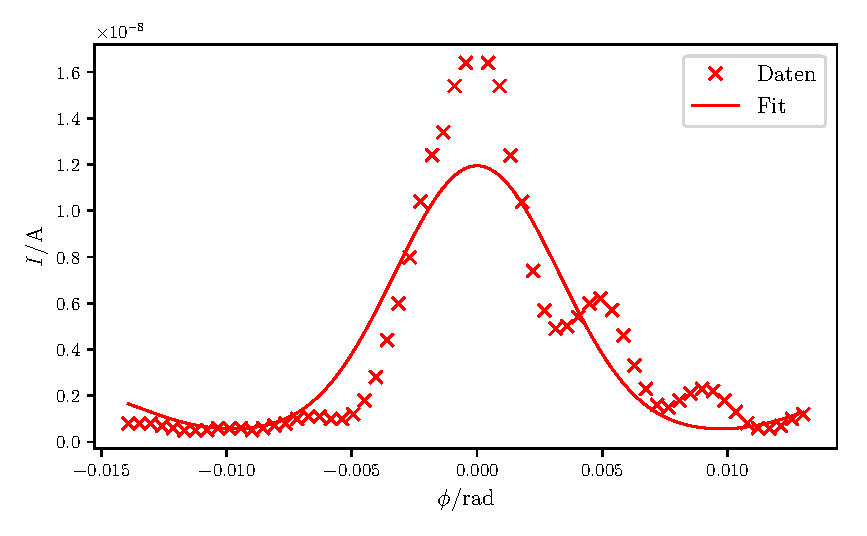
\includegraphics[width=15cm, height=9cm]{build/plot1.pdf}
    \caption{Die Werte aus Tab. \ref{tab1} gegeneinander aufgetragen.
    Zu sehen ist das Beugungsbild eines Einzelspalts.}
    \label{fig:plot1}
\end{figure}

\noindent Mit Hilfe einer Ausgleichsrechnung und der Gleichung \eqref{eqn:intensität} lassen sich die Parameter $A_0$, $b$ und $d$ bestimmen, wobei $A_0$ die Amplitude angibt, $b$ der Breite des Spalts und $d$ dem Wert des Off-Stroms während des Experiments entspricht. 

\noindent Für die Werte gilt
\begin{align*}
    A_0 &= \SI{-0.899(055)}{\ampere\per\meter} \\
    b &= \SI{-78.07 \pm 2.88}{\micro\meter} \\
    d &= \SI{1.53(15)}{\nano\ampere}.
\end{align*}

\noindent Der Literaturwert für die Breite des Spalts beträgt
\begin{equation*}
    b_\text{lit,1} = \SI{150}{\micro\meter}.
\end{equation*}

\noindent Der gemessene Wert für den Off-Strom beträgt 
\begin{equation*}
    d_\text{gemessen}= \SI{1.6}{\nano\ampere}.
\end{equation*}


\subsection{Messung am zweiten Einzelspalt}
In Tab. \ref{tabb} befindet sich die $x$-Koordinaten in Einheiten der Messanzeige und die Amplituden der Stromstärke gegeneinander aufgetragen. 

\begin{table}\caption{Die angelegte Spannung des elektrischen Feldes innerhalb des Geiger-Müller-Zählrohrs, die Anzahl der jeweils gemessenen Impulse und der Strom innerhalb des Geiger-Müller-Zählrohrs.}
\label{tabb}
\centering
\sisetup{round-mode = places, round-precision=2, round-integer-to-decimal=true}
\begin{tabular}{c c S[]} 
\toprule
{$U / \si{\volt}$} & {$\frac{N}{\SI{130}{\second}}$} & {$I / \si{\ampere}$}\\
\midrule
320 & 11298 & 0.1\\
400 & 11820 & 0.2\\
480 & 12135 & 0.3\\
540 & 12301 & 0.35\\
560 & 12068 & 0.4\\
600 & 12354 & 0.45\\
640 & 12403 & 0.5\\
660 & 12507 & 0.55\\
680 & 12659 & 0.6\\
\bottomrule
\end{tabular}\end{table}

\noindent In Tab. \ref{tab2} werden die $x$-Koordinaten mit Gleichung \eqref{eqn:phi} in Winkel umgerechnet und gegen die Amplitude der Stromstärke aufgetragen. 

\begin{table}\caption{Das Verhältnis des magnetischen Feldes durch die Beschleunigungsspannung aufgetragen gegen die Höhe.}
\label{tab2}
\centering
\sisetup{round-mode = places, round-precision=2, round-integer-to-decimal=true}
\begin{tabular}{S[]S[]S[]} 
\toprule
{$B_1 / \si{\henry}$} & {$B_2 / \si{\henry}$} & {$\frac{D}{(L^2 + D^2)} / \si{\per\meter}$}\\
\midrule
0.0 & 0.0 & 0.0\\
3.5649278338607584e-07 & 3.862005153349155e-07 & 0.29289724188430566\\
8.912319584651897e-07 & 8.912319584651897e-07 & 0.5827222842713544\\
1.4259711335443034e-06 & 1.396263401595464e-06 & 0.8665094112549946\\
1.9250610302848096e-06 & 1.8418793808280586e-06 & 1.1414982164090373\\
2.3885016486867084e-06 & 2.3172030920094934e-06 & 1.4052180429996723\\
2.923240823765822e-06 & 2.822234535139767e-06 & 1.6555530006898145\\
3.4223307205063282e-06 & 3.3272659782700412e-06 & 1.8907846756403912\\
\bottomrule
\end{tabular}\end{table}

\noindent In Abb. \ref{fig:plot2} werden die Werte aus Tab. \ref{tab2} gegeneinander aufgetragen und es wird ein Fit in die Werte gelegt. 
\begin{figure}
    \centering
    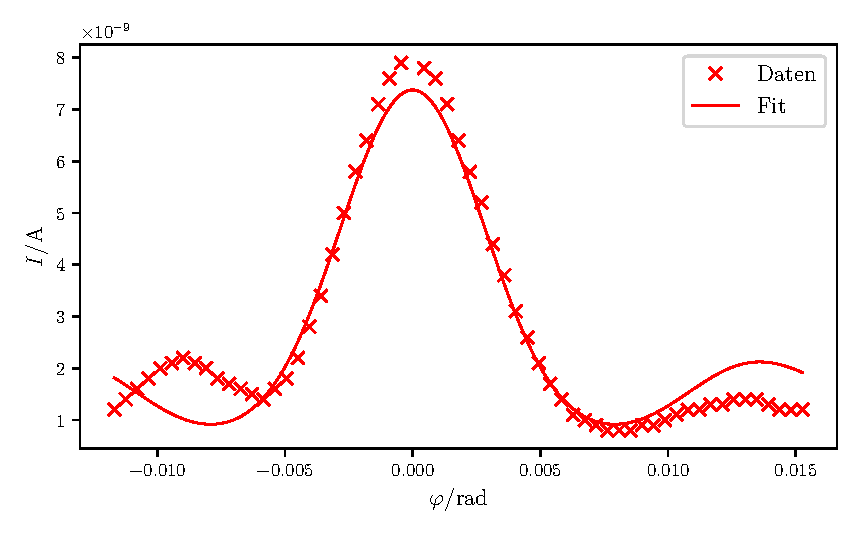
\includegraphics[width=15cm, height=9cm]{build/plot2.pdf}
    \caption{Die Werte aus Tab. \ref{tab2} gegeneinander aufgetragen.
    Zu sehen ist das Beugungsbild eines Einzelspalts.}
    \label{fig:plot2}
\end{figure}

\noindent Mit Hilfe einer Ausgleichsrechnung lassen sich wieder die Parameter $A_0$, $b$ und $d$ bestimmen. 

\noindent Für die Werte gilt
\begin{align*}
    A_0 &= \SI{0.4746 (023)}{\ampere\per\meter} \\
    b &= \SI{96.24 \pm 2.56}{\micro\meter} \\
    d &= \SI{1.62(07)}{\nano\ampere}. 
\end{align*}

\noindent Der Literaturwert für die Breite des Spalts beträgt
\begin{equation*}
    b_\text{lit,2} = \SI{75}{\micro\meter}.
\end{equation*}


\subsection{Beugung am Doppelspalt}
In Tab. \ref{tabc} befinden sich  die $x$-Koordinaten in Einheiten der Messanzeige und die Amplituden der Stromstärke gegeneinander aufgetragen. 

\begin{table}\caption{Der Anodenstrom und der Kathodenstrom bei einer Beschleunigungsspannung von $U_\text{B} = \SI{25}{\kilo\volt}$ und einer Kathodenspannung $U_\text{K,1} = \SI{500}{\volt}$ und einer Kathodenspannung $U_\text{K,2} = \SI{300}{\volt}$ bei einem Blendenradius von $r_\text{B} = \SI{5}{\milli\meter}$.}
\label{tabc}
\centering
\sisetup{round-mode = places, round-precision=2, round-integer-to-decimal=true}
\begin{tabular}{S[]S[]S[]} 
\toprule
{$I_\text{K} / \si{\milli\ampere}$} & {$I_\text{K,1} / \si{\nano\ampere}$} & {$I_\text{K,2} / \si{\nano\ampere}$}\\
\midrule
1.0 & 2.6 & 2.4\\
0.95 & 2.5 & 2.4\\
0.9 & 2.4 & 2.2\\
0.85 & 2.3 & 2.1\\
0.8 & 2.2 & 2.0\\
0.75 & 2.1 & 1.9\\
0.7 & 1.9 & 1.8\\
0.65 & 1.8 & 1.6\\
0.6 & 1.6 & 1.5\\
0.55 & 1.5 & 1.4\\
0.5 & 1.4 & 1.3\\
0.45 & 1.2 & 1.2\\
0.4 & 1.1 & 1.0\\
0.35 & 0.9 & 0.9\\
0.3 & 0.8 & 0.8\\
0.25 & 0.6 & 0.6\\
0.2 & 0.5 & 0.5\\
0.15 & 0.4 & 0.4\\
0.1 & 0.1 & 0.2\\
0.05 & 0.1 & 0.1\\
\bottomrule
\end{tabular}\end{table}

\noindent In Tab. \ref{tab3} werden die $x$-Koordinaten mit Gleichung \eqref{eqn:phi} in Winkel umgerechnet und gegen die Amplitude der Stromstärke aufgetragen. 

\begin{table}\caption{Der Winkel \varphi gegen die Stromstärke I aufgetragen.}
\label{tab1}
\centering
\sisetup{round-mode = places, round-precision=2, round-integer-to-decimal=true}
\begin{tabular}{S[]S[]} 
\toprule
{$\varphi / \si{\milli\radian}$} & {$I / \si{\nano\ampere}$}\\
\midrule
-12.577953012282642 & 1.0999999999999999\\
-12.353369766296458 & 0.8999999999999998\\
-12.128785274090491 & 1.1999999999999995\\
-11.904199558309829 & 1.7\\
-11.679612641600295 & 1.8\\
-11.455024546608442 & 1.1999999999999995\\
-11.230435295981538 & 1.1999999999999995\\
-11.005844912367545 & 1.8\\
-10.781253418415117 & 2.499999999999999\\
-10.556660836773576 & 1.9000000000000001\\
-10.332067190092905 & 1.1999999999999995\\
-10.107472501023729 & 1.6000000000000003\\
-9.882876792217305 & 2.9000000000000004\\
-9.658280086325508 & 3.1000000000000005\\
-9.433682406000813 & 1.8\\
-9.20908377389629 & 1.1999999999999995\\
-8.984484212665583 & 2.3\\
-8.759883744962893 & 3.6\\
-8.53528239344298 & 2.9000000000000004\\
-8.310680180761132 & 1.6000000000000003\\
-8.086077129573162 & 1.6000000000000003\\
-7.861473262535383 & 2.9000000000000004\\
-7.636868602304612 & 3.1000000000000005\\
-7.41226317153814 & 2.0\\
-7.187656992893724 & 1.4000000000000001\\
-6.963050089029578 & 2.1\\
-6.738442482604351 & 2.6\\
-6.513834196277122 & 1.9000000000000001\\
-6.289225252707374 & 1.2999999999999996\\
-6.064615674554994 & 1.6000000000000003\\
-5.840005484480253 & 2.4\\
-5.61539470514379 & 2.3\\
-5.3907833592066 & 1.6000000000000003\\
-5.166171469330024 & 1.6000000000000003\\
-4.941559058175732 & 2.4\\
-4.716946148405708 & 3.3000000000000007\\
-4.492332762682237 & 3.7\\
-4.2677189236678945 & 3.1999999999999997\\
-4.043104654025528 & 3.1000000000000005\\
-3.8184899764182507 & 4.199999999999999\\
-3.5938749135094157 & 6.1000000000000005\\
-3.369259487962614 & 7.599999999999999\\
-3.1446437224416557 & 6.599999999999999\\
-2.920027639610556 & 5.6000000000000005\\
-2.6954112621335216 & 7.000000000000001\\
-2.4707946126749376 & 10.4\\
-2.2461777138993564 & 12.400000000000002\\
-2.0215605884714787 & 10.4\\
-1.7969432590561418 & 8.399999999999999\\
-1.572325748318309 & 10.4\\
-1.3477080789230522 & 15.399999999999999\\
-1.123090273535539 & 16.400000000000002\\
-0.8984723548210195 & 13.4\\
-0.673854345444813 & 10.4\\
-0.44923626807229305 & 13.4\\
-0.22461814536887456 & 17.4\\
0.22461814536887456 & 13.4\\
0.44923626807229305 & 11.4\\
0.673854345444813 & 14.4\\
0.8984723548210195 & 17.4\\
1.123090273535539 & 15.399999999999999\\
1.3477080789230522 & 11.4\\
1.572325748318309 & 10.4\\
1.7969432590561418 & 12.400000000000002\\
2.0215605884714787 & 14.4\\
2.2461777138993564 & 11.4\\
2.4707946126749376 & 8.399999999999999\\
2.6954112621335216 & 8.399999999999999\\
2.920027639610556 & 10.4\\
3.1446437224416557 & 9.400000000000002\\
3.369259487962614 & 6.800000000000001\\
3.5938749135094157 & 5.5\\
3.8184899764182507 & 7.400000000000001\\
4.043104654025528 & 8.200000000000001\\
4.2677189236678945 & 6.2\\
4.492332762682237 & 4.199999999999999\\
4.716946148405708 & 4.9\\
4.941559058175732 & 6.599999999999999\\
5.166171469330024 & 6.1000000000000005\\
5.3907833592066 & 4.300000000000001\\
5.61539470514379 & 4.1000000000000005\\
5.840005484480253 & 5.6000000000000005\\
6.064615674554994 & 6.0\\
6.289225252707374 & 4.7\\
6.513834196277122 & 4.1000000000000005\\
6.738442482604351 & 5.2\\
6.963050089029578 & 5.9\\
7.187656992893724 & 4.9\\
7.41226317153814 & 3.8000000000000003\\
7.636868602304612 & 4.4\\
7.861473262535383 & 5.4\\
8.086077129573162 & 4.9\\
8.310680180761132 & 3.3000000000000007\\
8.53528239344298 & 2.9999999999999996\\
8.759883744962893 & 3.8000000000000003\\
8.984484212665583 & 3.9999999999999996\\
9.20908377389629 & 2.9999999999999996\\
9.433682406000813 & 2.0\\
9.658280086325508 & 2.0\\
9.882876792217305 & 2.3\\
10.107472501023729 & 2.0\\
10.332067190092905 & 1.5000000000000002\\
10.556660836773576 & 1.2999999999999996\\
10.781253418415117 & 1.0999999999999999\\
11.005844912367545 & 0.9999999999999999\\
11.230435295981538 & 0.8999999999999998\\
11.455024546608442 & 0.9999999999999999\\
11.679612641600295 & 0.9999999999999999\\
11.904199558309829 & 0.8999999999999998\\
12.128785274090491 & 0.6999999999999996\\
12.353369766296458 & 0.6999999999999996\\
12.577953012282642 & 0.8999999999999998\\
12.802534989404709 & 1.0999999999999999\\
13.027115675019099 & 1.0999999999999999\\
13.251695046483025 & 0.8999999999999998\\
13.476273081154504 & 0.6999999999999996\\
13.70084975639236 & 0.9999999999999999\\
13.925425049556234 & 1.2999999999999996\\
14.14999893800661 & 1.2999999999999996\\
14.374571399104815 & 0.9999999999999999\\
\bottomrule
\end{tabular}\end{table}

\noindent In Abb. \ref{fig:plot4} werden die Werte aus Tab. \ref{tab3} gegeneinander aufgetragen, es wird ein Fit in die Werte gelegt
und eine Theoriekurve eingetragen. 

\begin{figure}
    \centering
    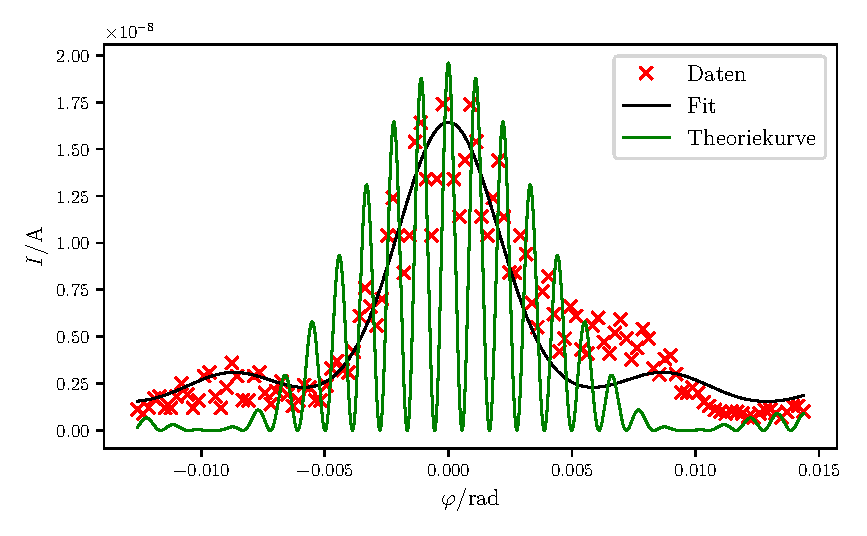
\includegraphics[width=15cm, height=9cm]{build/plot4.pdf}
    \caption{Die Werte aus Tab. \ref{tab3} gegeneinander aufgetragen.
    Zu sehen ist das Beugungsbild eines Doppelspalts mit dem Fit
    als Einhüllende und einer Theoriekurve.}
    \label{fig:plot4}
\end{figure}

\noindent Mit Hilfe einer Ausgleichsrechnung lassen sich wieder die Parameter $b$, $s$, $A$ und $d$ mit Gleichung \eqref{eqn:doppelspalt} bestimmen. Dieses mal aber für den Doppelspalt. 

\noindent Für die Werte gilt
\begin{align*}
    b &= \SI{101.820 \pm 5.293}{\micro\meter} \\
    s &= \SI{40.29 \pm 3.69}{\micro\meter} \\
    A &= \SI{39.43 \pm 1.91}{\micro\ampere} \\
    d &= \SI{2.44(21)}{\nano\ampere}. 
\end{align*}

\noindent Aus der Theoriekurve ergeben sich folgende Werte
\begin{align*}
    b &= \SI{55}{\micro\meter} \\
    s &= \SI{480}{\micro\meter} \\
    d &= \SI{1.6}{\nano\ampere}.
\end{align*}
Die Amplitude ergibt sich zu 
\begin{equation*}
    A = \SI{70}{\micro\ampere}. %Einheit richtig? Ja, perfekt.
\end{equation*}

\noindent Der Literaturwert für die Breite der beiden Spalten beträgt
\begin{equation*}
    b_{\text{lit}} = \SI{100}{\micro\meter}
\end{equation*}
und für den Spalt 
\begin{equation*}
    s_{\text{lit}} = \SI{200}{\micro\meter}.
\end{equation*}
